% LaTeX style file for Ph.D. thesis document
% Institution: Kyungpook National University (KNU)
% 
% (c) Gwenaelle Cunha Sergio (gwena.cs@gmail.com)
% and
% (c) Dennis Singh Moirangthem (mdennissingh@gmail.com)
%
% Please note:
%    1. Compile with XeLatex
%    2. This was not made for monetary purposes and it is free for anyone to use. However, if you do use it or modify it, please acknowledge this work by mentioning this original source code.
%

\documentclass[12pt]{article}

\usepackage{thesis}
%%%%%%%%%%%%%%%%%%%%%
% Required packages %
%%%%%%%%%%%%%%%%%%%%%

% Document formatting
\usepackage{adjustbox}
\usepackage{ragged2e}
\usepackage{setspace}
\usepackage{times}
\usepackage{latexsym}
\usepackage{url}
\usepackage{etoolbox}
\usepackage{graphicx}
\usepackage{url}
\usepackage{amsmath}
\usepackage{amssymb}
%\usepackage{subfigure}
\usepackage{color}
\usepackage{multirow}
\usepackage{comment}
\usepackage{pdflscape}
\usepackage{bibentry}
\usepackage{caption}
\usepackage{booktabs}
\usepackage[noadjust]{cite}
\usepackage{fancyhdr}



% Needed for \phantomsection definition
\usepackage{hyperref}

% Images
\usepackage{graphicx}
\usepackage{subfig}

% Indents first paragraph
\usepackage{indentfirst}

% Suppress badness warnings
\hbadness=99999


%%%%%%%%%%%%%%%%%%%%%%
% Thesis information %
%%%%%%%%%%%%%%%%%%%%%%

\title{Thesis title line 1\\ Title line 2}
\author{Your English Name}
\supervisor{Prof. 1 \\Co-supervised by Professor Prof. 2}
\department{School of Electronics Engineering, Major in Signal Processing}
\profA{Prof. 1}
\profB{Prof. 2}
\profC{Prof. 3}
\profD{Prof. 4}
\profE{Prof. 5}

\titlekorean{Title in Korean}
\authorkorean{한국 이름 (Your Korean Name)}
\supervisorkorean{지도교수 이름 (Prof. 1 Name in Korean) \\공동지도교수 (Prof. 2 Name in Korean)}
\departmentkorean{경북대학교 대학원 전자공학부 신호처리전공}

%%%%%%%%%%%%%%%%%%%%%%%%
% Document starts here %
%%%%%%%%%%%%%%%%%%%%%%%%
\begin{document}

\makecover
\makeinnercover
\pagebreak

\pagenumbering{roman} %\frontmatter
\setstretch{1.5}

\setcounter{secnumdepth}{5}
\setcounter{tocdepth}{3}
\titleformat{\paragraph}
{\normalfont\normalsize\bfseries}{\theparagraph}{1em}{}
\titlespacing*{\paragraph}
{0pt}{3.25ex plus 1ex minus .2ex}{1.5ex plus .2ex}

\titleformat{\subparagraph}
{\normalfont\normalsize\bfseries}{\thesubparagraph}{1em}{}
\titlespacing*{\subparagraph}
{0pt}{3.25ex plus 1ex minus .2ex}{1.5ex plus .2ex}

\renewcommand{\cftsecaftersnum}{.}
\renewcommand{\cftsecleader}{\cftdotfill{\cftdotsep}}
\renewcommand{\contentsname}{\begin{center}Contents\end{center}}
\tableofcontents \pagebreak
\setlength{\cftfigindent}{0pt}
\setlength{\cfttabindent}{0pt}
\renewcommand{\cftfigpresnum}{Figure~}
\renewcommand{\cftfignumwidth}{5em}
\renewcommand{\cfttabpresnum}{Table~}
\renewcommand{\cfttabnumwidth}{4.5em}


\listoffigures \pagebreak

\listoftables \pagebreak
\setlength{\footskip}{40pt} %set page number distance from content
\pagenumbering{arabic} %\mainmatter

%hyphen page numbers
\fancypagestyle{plain}{%
  \fancyhf{}%
  \fancyfoot[C]{\fontsize{10pt}{10pt}\selectfont-~\thepage~-}% set font to 10
  \renewcommand*{\headrulewidth}{0pt}%
  \renewcommand*{\footrulewidth}{0pt}%
}
\pagestyle{plain}

\setstretch{1.85}  % Times New Roman 12pt
\renewcommand{\thefigure}{\arabic{section}.\arabic{figure}}
\renewcommand{\thetable}{\arabic{section}.\arabic{table}}
\justifying
\setcounter{figure}{0}
\setcounter{table}{0}
\section{Introduction}~\label{sec:introduction}
This is the template for the PhD thesis of School of Electronics Engineering, KNU. Please check and confirm your department name with the office.

You change the month and year of graduation from `June 2020' to yours in thesis.sty.

The remainder of this thesis is organized as follows. The subsections, figures, and tables are described in Chapter~\ref{sec:subsections}. The equations are described in Chapter~\ref{sec:equations}. Section~\ref{sec:add_ref} explains how to add the references. Finally, the conclusions and the future directions are detailed in Chapter~\ref{sec:conclusion}.
 \pagebreak
\setcounter{figure}{0}
\setcounter{table}{0}
\section{Sub Sections, Figures and Tables}~\label{sec:subsections}

In this chapter, how to the subsections and also the tables and figures are discussed in detail.

\subsection{Sub Section}\label{sec:subsection}
An example table is shown in Table~\ref{tab:dataset}.

\begin{table}[!ht]
\center
\caption{An example table.}
\label{tab:dataset}
\begin{tabular}{lccc}
\hline
Dataset Name& Classes & Training Set & Testing Set\\ \hline
Yelp P& $2$ & $560,000$ & $38,000$ \\
Yelp F& $5$ & $650,000$ & $50,000$ \\ 
Yahoo& $10$ & $1,400,000$ & $60,000$ \\  
Amazon F & $5$ & $3,000,000$& $650,000$ \\
Amazon P & $2$ & $3,6000,000$ & $400,000$ \\
DBPedia& $14$ & $560,000$ & $70,000$  \\
\hline
\end{tabular}
\end{table}


\subsubsection{Sub Sub Section}\label{sec:subsubsection}

An example figure is shown in Figure~\ref{fig:dataset}.

\begin{figure}[ht!]
    \centering
    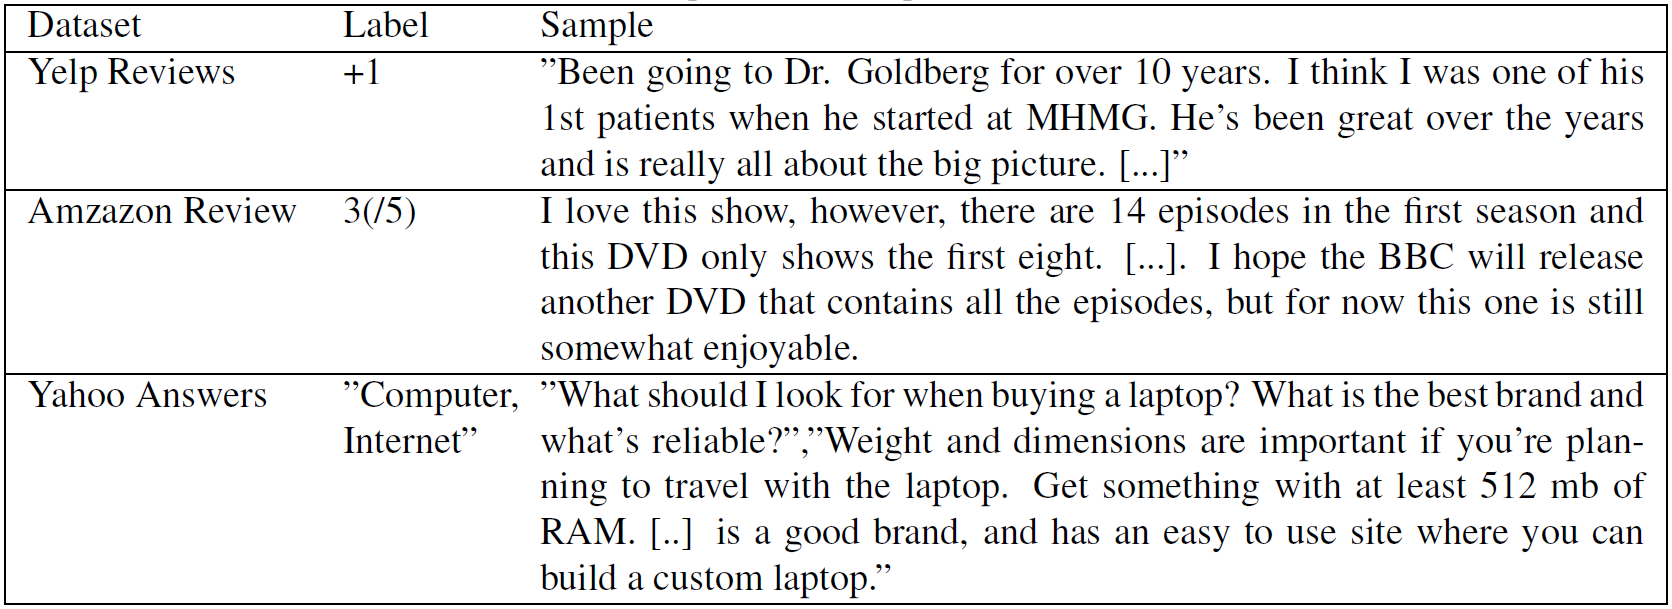
\includegraphics[width=1\columnwidth]{figures/dataset.png}
    \caption{An example figure.}
    \label{fig:dataset}
    \vspace{-3mm}
\end{figure}

 
\paragraph{Sub Sub Sub Section}\label{sec:subsubsubsection}
This is a Sub Sub Sub Section. This will not show up in the table of contents (TOC). If you want it to be shown, then set the ``tocdepth'' to 4 or more in thesis.tex.

\subparagraph{Sub Sub Sub Sub Section}\label{sec:subsubsubsubsection}
This is a Sub Sub Sub Sub Section. This will not show up in the TOC. If you want it to be shown, then set the ``tocdepth'' to 5 in thesis.tex. \pagebreak
\setcounter{figure}{0}
\setcounter{table}{0}
\section{How to add an equation}~\label{sec:equations}

An example Eq.~\eqref{eqn:gru} is as follows.  
\begin{equation}
\vspace{0mm}
\begin{aligned}
\label{eqn:gru}
& r_t = \sigma( W_{xr} x_t + W_{hr} h_{t-1}) \\
& z_t = \sigma( W_{xz} x_t + W_{hz} h_{t-1}) \\
& u_t = \tanh( W_{xu} x_t + W_{hu} (  r_t \odot h_{t-1}))\\
& h_t =  z_t h_{t-1} + (1 - z_t) u_t\\
\end{aligned}
\vspace{0mm}
\end{equation}
where $\sigma(\cdot)$ and $\mbox{tanh}(\cdot)$ are the sigmoid and tangent hyperbolic activation functions, respectively, $\odot$ denotes the element-wise multiplication operator,
and $\mathbf{r}_t$,  $\mathbf{z}_t$ are referred to as {\em reset}, {\em update} gates, respectively. $\mathbf{u}_t$ and  $\mathbf{h}_t$ are the candidate activation and the new hidden state of the GRU, respectively. \pagebreak
\setcounter{figure}{0}
\setcounter{table}{0}
\section{Adding References}\label{sec:add_ref}

This is a reference to a section: We use the data described in Section~\ref{sec:subsection}.

\subsection{Example references}
For evaluation, the Recall-Oriented Understudy for Gisting Evaluation (ROUGE) metrics~\cite{lin2004rouge} proposed by Lin et al.~\cite{lin2003automatic} is adopted.
 \pagebreak
\section{Conclusion and Future Works}~\label{sec:conclusion}

\lipsum[3] \pagebreak

%\section*{References}
\setstretch{1.0}
\phantomsection~\label{sec:ref}
\addcontentsline{toc}{section}{References}
\bibliographystyle{IEEEtran}
\bibliography{bibliography.bib}
\pagebreak

% ABSTRACT IN ENGLISH
\phantomsection~\label{sec:abstract_english}
\addcontentsline{toc}{section}{Abstract (In English)}

% Make header
\makeabstractheader

% Abstract text
\setstretch{1.85}
\lipsum[5]
 \pagebreak
% ABSTRACT IN KOREAN
% Add it to Contents
\phantomsection~\label{sec:abstract_korean}
\addcontentsline{toc}{section}{Abstract (In Korean)}

% Text is lipsum, generated with https://generator.lorem-ipsum.info/_korean

% Make header
\makeabstractheaderkorean

% Abstract text
\setstretch{1.85}
대통령이 궐위되거나 사고로 인하여 직무를 수행할 수 없을 때에는 국무총리, 국회의원은 그 지위를 남용하여 국가·공공단체 또는 기업체와의 계약이나 그 처분에 의하여 재산상의 권리·이익 또는 직위를 취득하거나 타인을 위하여 그 취득을 알선할 수 없다, 중임할 수 없다, 1차에 한하여 중임할 수 있다.

우호통상항해조약. 1차에 한하여 중임할 수 있다, 이 헌법시행 당시의 법령과 조약은 이 헌법에 위배되지 아니하는 한 그 효력을 지속한다. 다만. \pagebreak

\end{document}